\documentclass{article}
\usepackage{amsmath}
\usepackage{graphicx}

\graphicspath{{../src}}

\title{Progress Report}
\author{Annabelle Cloutier}


\begin{document}
\maketitle

\tableofcontents

\section{Paper}

\subsection{Network Structure}

All of the below is based on the work in \cite{eco-dqn}
The network structure is incredibly generic most of the way through, but notes are written here to avoid having to parse through the equations that describe the network structure in the paper. Note that at any step where learned weights are used, the ReLU function is used on the resulting vector. The only exception is for the last set of learned weights in the readout layer.

\subsubsection{Node Embedding}\label{node-embedding}

The MPNN (Message Passing Neural Network) structure used converts each vertex into a set of $m$ observations and encodes them into a $n$-dimensional embedding using learned weights. The paper states that they use 64 dimensional embeddings and they do in code, but this could be any size. 

The observations in the paper as well as their justifications for them are as follows: 

\begin{enumerate}
    \item Whether the current vertex belongs to the solution set $S$ or not; 
    
    This is a local observation. The reason they state this observation is important is that it provides useful information for the agent to make a decision on whether the vertex should be added or removed from the solution set.

    \item The immediate cut change if the current vertex state is changed;
    
    This is also a local observation. Just as with the above observation, they state this provides useful information for decision making. They also state is that it allows the agent to exploit having reversible actions. This makes intuitive sense, as knowing the difference between having a vertex in the solution or not can allow the agent to make an informed decision on whether to add or remove it, or in this agent's case, possibly reversing an action. 

    \item The number of steps since the current vertex state was changed;
    
    Also a local observation. For this observation, they mention that it provides a simple history to the agent to prevent looping decisions. Because this observation gets larger as time goes on and a vertex is unchanged, the agent will be further incentivised to choose other vertices if it gets stuck in a loop choosing the same few vertices over and over. They also state it allows the agent to exploit reversible actions just as with observation 2. This specific observation could be important as the value increases as the vertex remains unchanged, which can entice the agent to choose vertices that have not been chosen in a long time to encourage exploration just as it will discourage loops.
    
    \item The difference of the current cut value from the best observed;
    
    This and all future observations are global. This observation they state ensures the rewards are Markovian. Just as with observations 2-4, this observation they also mention allows the agent to exploit having reversible actions, which makes intuitive sense. The agent knowing the difference between the current cut value and the best one observed, along with the other observations, can allow the network to make informed decisions on whether the current solution is a promising set to explore.

    \item The distance of the current solution set from the best observed;
    
    This observation as with observation 5 they state ensures the rewards are Markovian. Again, this observation allows the agent to exploit reversible actions. 

    The difference between this and observation 5 is that observation 5 compares the cut value only. This observation compares the solution sets and counts the number of vertices that differ between the best observed solution set of vertices and the current one. This is not explained in the paper, but can be seen in the code, specifically in src/envs/spinsystem.py, in the SpinSystemBase class' step function.

    Example for clarity:

    Best seen bitmask of vertices: $[0, 0, 1, 0, 1]$

    Current bitmask of vertices: $[0, 1, 1, 0, 1]$.

    Difference: 1. 

    Counting the number of different vertices they do in code by subtracting the two and counting the number of non-zero values. This can also be done using a bitwise XOR and doing a sum on the resulting bitmask. 

    \item The number of available actions that immediately increase the cut value;
    
    Once again, this observation ensures Markovian rewards, they also mention that this allows exploitation of reversible actions, which is more easily understandable.

    \item The number of steps remaining in the episode
    
    The only reasoning they have for this observation is that it accounts for the finite time used for solution exploration. 

\end{enumerate}

\subsubsection{Edge Embedding}

The edges for each vertex are also encoded into a separate $n$-dimensional embedding, same size as for each vertex, once again learned. The input for this step is the set of $m$ observations of the neighboring vertices catenated with the weight on the connecting edge, creating an $m + 1$ dimensional vector for each neighboring vertex. All of these vectors are then summed and passed through a learned layer, creating an $n - 1$ dimensional vector. At this stage, the resulting $n - 1$ dimensional vector is divided by the number of neighbors, catenated with the number of neighbors, and passed through another learned layer, resulting in an $n$-dimensional embedding representing the edges for a vertex.

The end result of these two steps are an $n$-dimensional embedding representing a vertex and another representing it's neighbors, all created using the same learned weights for every vertex. Meaning there will be $2|V|$, $n$-dimensional embeddings. 


\begin{enumerate}
    \item Why 64 dimensions on the vertex and edge embeddings? 
    
    It's nice that it's 64 but finding the reason why will be important to make informed decisions on modifying the network.
\end{enumerate}

\subsubsection{Message Passing}

Here there is a message pass layer and an update layer. The message pass per vertex is summing the products of the connected vertices and the weight, divided by the number of neighbors, catenated with the edge embedding for that vertex and then passed through learned weights, resulting in a $n$-dimensional vector.

The next is the update layer, which is the embedding for that vertex, catenated with the message and passed through another set of learned weights, into an $n$-dimensional vector, representing the "new" embedding for that vertex. 

The message then update is performed $K$ times. Mentioned in the paper and corroborated in the code, this is done 3 times, but can be done however many times necessary.

\begin{enumerate}
    \item Why have new network layers for these steps?
    
    As with the decision on the hidden layers sizes, understanding the justification for why certain steps are passed through learned functions before more calculations are performed will help make informed decisions on network changes.
\end{enumerate}

\subsubsection{Readout}

The readout layer goes through each vertex, summing the embeddings for the neighbors of that vertex, dividing the result by the number of vertices in the entire graph and then passing it through learned weights, resulting in an $n$-dimensional vector.

The embedding for the vertex itself is then catenated to the resulting vector and passed through another set of learned weights (without applying ReLU), giving in a single output value. This value represents the Q-value for that vertex, which is used by the algorithm to determine which vertex will be added/removed from the solution set on that step. The vertex associated to the maximum Q-value is added to the solution set if it doesn't yet belong to it, or removed from the solution set if it belongs to it.

\subsection{Reward Shaping and Training}

\subsubsection{Q Function, Q values and Training}

The Q function is an idea derived from Q-learning \cite{qlearning} which proposes a way for an agent to learn how to behave in an environments. It is defined as the expected value of the discounted sum of future rewards for any state-action pair of an environment. When an optimal Q function is derived, the agent chooses which action to perform in a certain state by selecting the state-action pair which corresponds to the largest Q-value, which is expected to give them to largest reward. The equation following equation represents this idea:
 
$Q^\pi(s, a) = E[\sum_{t=0}^{\infty} \gamma^t R(s_t) | s_0 = s, a_0 = a, \pi]$

where $\pi$ is a policy, mapping a state to a probability distribution over the actions, $R(s)$ is the reward for a given state and $\gamma^t$ is a discount given to change whether the agent prefers immediate or future rewards.

This Q function is learned by a Markov decision process. The agent traverses the environment and rewards are given at each step depending on the result of the action the agent performs.

Trying to find this Q function was known to be unstable or even diverge when nonlinear function approximators, like neural networks, were used to try and represent it \cite{td-func-approx}. In \textit{Mnih et al.}, they propose an approach to Q learning with two main ideas; namely experience replay and an iterative update, adjusting the Q values towards target values only periodically \cite{deepmind_2015}. The agent during training only chooses the actions associated with its current policy with probability $1 - \epsilon$ and otherwise chooses a random action. They demonstrate experimentally that with these ideas, they were able to train a model that had significant performance improvements compared to other existing models on 49 different Atari games.

These ideas are replicated in the training of ECO-DQN. For every episode in the training phase, a random graph is sampled with a random solution set. Then, for each time step in that episode, the agent chooses a random vertex based on the existing Q function with a probability $\epsilon$ and a vertex dictated by it's Q function otherwise. Then, the starting state, chosen vertex, reward and resulting state are added to the experience replay memory. Finally, after some fixed set of time steps, the network is updated by stochastic gradient descent on a minibatch sampled from the experience replay memory.

\subsubsection{Reward Shaping}

The reward in a certain state is given by the difference between the cut value in that state and the highest cut value seen so far in the episode, divided by the number of vertices. If the difference is negative, it's instead set to 0. The justification behind this choice is that a negative reward will discourage the agent from exploring states that give an immediately worse cut value, even if other cuts including that change later on may give better cut values. If this were to happen, it would discourage the agent from exploring different cut values and cause it to stay in a very small space near a locally maximal cut value. Because previously seen optimal states are stored in memory, it's beneficial to later let the agent explore more states in an attempt to find more locally optimal states, even if not always better than the previously seen local optimum.

They also define a reward for reaching locally optimal states of $\frac{1}{|V|}$. This is once again to encourage exploration. Because the previously seen best cut is stored, it's beneficial for the agent to explore other states, even if other local optimums may be worse than the previously found best cut. They state that local optima in combinatorial problems are typically close to each other and therefore by giving rewards for reaching new local optimums, the agent learns to hop between them during training as it is rewarded for this behaviour. Without this, they state that because there are far too many states to be visited in a finite time, which is typical for combinatorial optimization problems, it is therefore useful to focus on these subsets of states near local optimums.

There is no exact reason stated for the choice of value, however it can be hypothesized that if a constant value is chosen, this could cause disproportionate reward shaping on different sized graphs. For example, graphs that have significantly more locally optimum cuts could end up rewarding the network too much for imply finding local optimums instead of attempting to find a global optimum, while using the exploration of local optimums as a means to that end. Larger graphs are likely to have more locally optimal states, it therefore makes sense to choose a value that decays as the size of the graph increases. Therefore a reward proportional to the inverse of the number of vertices in the graph therefore makes the most sense. 

The choice to not randomly change states when a new local optimum is found appears to be mostly a choice that the authors made intentionally as they want the network to find some space that has numerous locally optimum states near each other to explore, and the best way to do this is to encourage finding nearby local optimums instead of sending the agent in different random directions every time a new local optimum is found. They do state that because there are far more states than can be visited within a finite time period, it's therefore more useful to find some local optimums that are near each other and explore that specific space of possible solutions.

They demonstrate this behaviour by observing the probability during any given timestep that the agent will either revisit a state, find a locally optimal state or find the maximum cut on the validation set. They show that as the number of timesteps goes up, the probability that the agent revisits a state goes up, as does the probability of finding the maximum cut, while the probability that the agent finds a local optimum goes up very quickly and stabilizes for the rest of the time steps, showing that the agent picks a certain set of local optimum and explores that space by revisiting previously seen states.

One thing this paper does not tackle is the issue of invalid solution states and how this would affect reward shaping, especially in a situation where the agent would be allowed to revert previously made actions. This isn't necessary for the Maximum Cut Problem, as any partition of the graph into two containing all vertices is a valid cut, but problems like the Traveling Salesman, Minimum Vertex Cover, Minimum Bisection  could possibly include states that are not valid solutions by either not being a complete path, not covering every vertex, having two sets of different sizes or having items that are not in a bin, respectively for each problem.

\subsection{Discussion on Generalization}

Most of the internal structure is generic for any graph, however because of the large number of changes that would likely need to be made to observations as well as the interpretation of the output for many other types of problems, it is likely that some changes to the internal structure would have to be made for the agent to make more educated decisions on new problems.

Everything outside of observations (input) and Q-values (output) only propagates information throughout the graph. This means the internal structure likely could remain mostly the same for any problem, so long as good decisions are made for the observations and that the output or it's interpretation are modified to fit new problems.

It is possible for more complex problems that some of the internal structure for the message and update sections of the network may have to change in order to accommodate for extra information. It is also possible that global observations could be embedded somewhere within the internal structure of the network instead of as input observations for every vertex.

The main issue comes with the output and it's interpretation. Each vertex is represented by a single value as the output, and that value is interpreted as adding or removing it from the solution set, in the context where the solution is a subset of the vertices in the graph. More specifically for the Max Cut problem, the vertex associated with the maximum Q-value (output value) is taken and then either added or removed from the solution set, depending on whether it already belongs to it or not. This approach works fine for a problem like Maximum Cut or Minimum Vertex Cover where the solution can be represented as a set representing chosen vertices for the solution, however any extra constraints forces the output interpretation to be completely redesigned. 

For example, the Traveling Salesman Problem where the solution is an ordered list of vertices would not correctly work as the current implementation of simply adding or removing a vertex from the solution could not work or would have to be changed significantly for this problem.

The Minimum K-Cut Problem which can have an arbitrary number partitions of the graph would also not work with the current model as it would require extra decision making on deciding which set to move a vertex to. Because the number of sets can also change, this means the size of the output would have to change as the solution changes which isn't possible, or some significant rework of the output interpretation would have to be made.

The Minimum Bisection Problem can be represented as a set of chosen vertices, however the extra constraint that the number of chosen vertices has to be the same as the number of unchosen vertices makes the current output interpretation incomplete for solving this problem. The same principle applies to the Minimum Vertex Cover, as it is possible to create invalid solutions for this problem. 

\subsection{Benchmarks}

The paper displays the performance of the graph in reference to S2V-DQN, a similar paper where the algorithm does not allow for reversing actions as well as a greedy algorithm. It also compares it's performance against modifications of itself, namely where some observations are restricted, intermediate rewards are not given for reaching locally optimal solutions, as well as keeping it from reversing its actions. 

They also include the MaxCutApprox algorithm, which is a greedy algorithm choosing the vertex that provides the greatest cut improvment until it can't improve the cut any more. They implement two variations of this, one where it can reverse actions and one where it can't. 

They also use an approximation ratio $C(S^*)/C(S_{opt})$. However, because $S_{opt}$ cannot be calculated exactly, they use multiple optimizations. Specifically, they use CPLEX, an integer programming solver, as well as a pair of simulated annealing heuristics by Tiunov \textit{et al.} (2019) and Leleu \textit{et al.} (2019) in order to calculate $S_{opt}$. 

The implementation of these different algorithms is not included in the codebase provided. However the optimal solutions and cut values for the ER graphs with 40 vertices are provided for the testing graphs. The validation graphs all have their maximum cut values included.

They use GSet graphs G1-10 and G22-32 as well as the Physics/Ising dataset as benchmark graphs. These, as well as their optimal cuts and solutions are provided in the codebase. 

\subsection{Graph Generation}

They train and test on Erdos-Renyi \cite{erdos} and Barabasi-Albert \cite{albert} graphs. For training, they generate random graphs and traverse them, adding each state, action and reward to the experience replay memory. For testing, they have a set of 50 graphs matching the parameters of the training graphs, being either ER or BA graphs with the same number of vertices.

\section{Code}

The code holds the capability of running all of the above tests, but they're not explicitly written and must be generated via self-written code.

\subsection{Running Code}

They very generously provide a README file that specifies the exact commands to run in order to train, test and validate networks. However, there is no code for reproducing their specific tests. These all need to be hand-coded. The only results I've reproduced so far are training and testing. These files can be modified easily to change where the network weights are stored, as well as the training result graphs and data. 

\subsection{Graph Generation}

Unsure of the exact implementation, it seems they use NetworkX's ability to generate random graphs in order to do this. For training, they use the classes defined in src/envs/utils to generate new graphs at each step, adding every action done on the new graphs to the experience replay memory which is used to train the network. This ensures every training session is random and includes different data. The testing graphs are all the same, but change depending on the size of the training networks. For example, a network trained on graphs with 40 vertices will also have it's performance tested on graphs with 40 vertices. 

\section{Minimum Cut}

The Minimum Cut is not an NP-Hard problem, but it is still a combinatorial optimization problem that could be solved by ECO-DQN. To confirm that the idea is expandable to other problems, we'll train an identical structure, using the negative of the cut value for determining the solution's reward with respect to the best observed, forcing the network to minimize the cut instead of maximize it. 

$R(S) = max(0, -C(S) - -C(S^*))$. 

\subsection{Results}

The result of training this network is very similar to the maximum cut. It starts giving random solutions and eventually reaches a point where the cut value found stabilizes on the test graphs. This demonstrates that the network structure can be utilized to solve other problems.

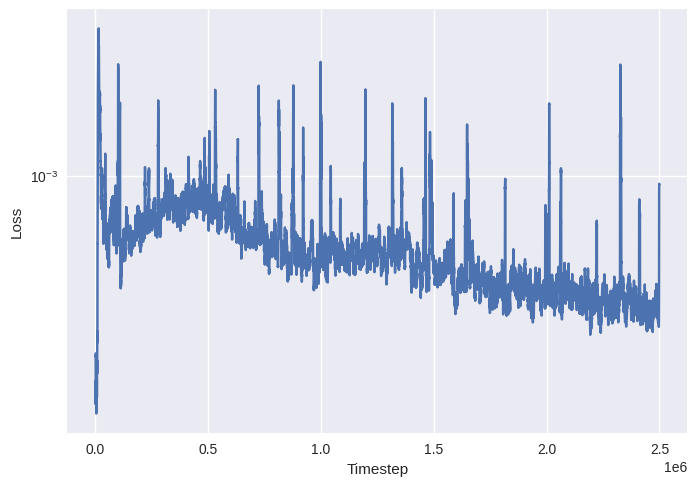
\includegraphics[scale=0.5]{../ER_20spin/eco/min_cut/network/loss.png}

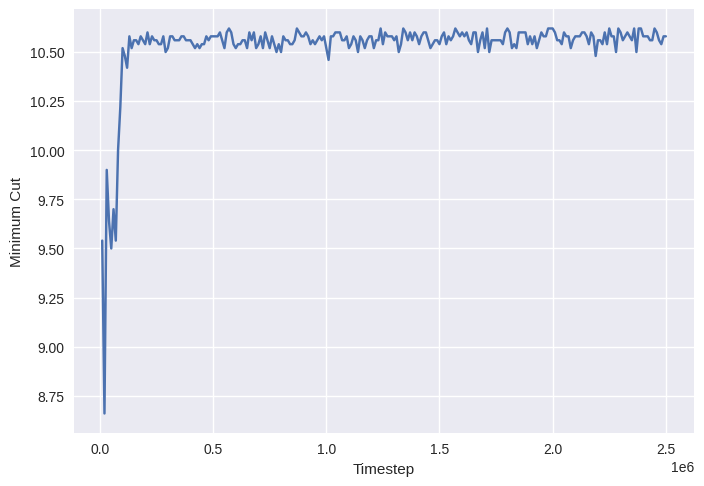
\includegraphics[scale=0.5]{../ER_20spin/eco/min_cut/network/training_curve.png}

This could be further tested to compare against existing algorithms for the Minimum Cut, but this at least shows promise.

\section{Minimum Vertex Cover}

A vertex cover is a set of vertices such that every edge in a graph has at least one endpoint in the that set of vertices. The vertex cover of smallest magnitude for a graph is known as the Minimum Vertex Cover. Finding this cover is known to be NP-hard. To tackle this issue with the approach in ECO-DQN, a few problems need to be solved:

\begin{enumerate}
    \item What observations will be used for each vertex 
    \item What will the reward be for finding a valid solution 
    \item What will be the punishment (if any) for finding sets that are invalid solutions 
    \item Should an intermediate reward be used for finding valid solutions that are locally optimal
    \item Should we allow invalid candidate solutions 
\end{enumerate}

Thankfully, some of these are somewhat trivial to solve, like the observations and reward, by either using ideas from ECO-DQN \cite{eco-dqn} and the similar S2V-DQN \cite{s2v-dqn} which does not allow for exploration/undoing actions but does tackle the Minimum Vertex Cover.

The last question we'll tackle in two parts. First, we'll attempt this problem by giving the network valid solutions and not allowing it to select invalid ones by severely penalizing those actions and randomizing a new solution to give it at test time to avoid the network getting stuck in local optimums in case it continuously tries to suggest invalid candidates.

\subsection{Observations}

In ECO-DQN, they have their set of observations from which we can draw to design the observations for the Minimum Vertex Cover. Some of these are even somewhat trivial to convert, namely:

\begin{itemize}
    \item Observation 1, "Vertex sate, i.e. if $v$ is currently in the solution set, $S$" is very easily translatable. We can directly copy this information, irrespective of if the current state is a valid solution.
    \item Observation 3 "Steps since the vertex state was last changed". This one also can be directly copied.
    \item Observation 4 "Difference of current cut-value from best observed". We will translate this to the difference between the current cover set size and the best cover set size. For this, we'll ignore the validity of the solution.
    \item Observation 5 "Distance of current solution set from the best observed". In the paper they do not define this, but it is explained through their implementation in Section \ref{node-embedding}, Node Embeddings. We can also use this information for the Minimum Vertex Cover in the same way.
    \item Observation 6 "Number of available actions that immediately increase the cut value" can also be translated. Namely, counting the number of actions (or vertices) that when flipped will reduce the number of vertices in the cover. Again, in this case we'll ignore the validity of the solution created by changing that vertex state.
    \item Observation 7 "Steps remaining in the episode". This, once again, can be directly copied.
\end{itemize}

Observation 2 in the ECO-DQN paper was the immediate cut change if the vertex state is changed. We would interpret this as the immediate change in the size of the vertex cover's set ignoring validity, but this is implied by Observation 1 for the Minimum Vertex Cover. 

With all of this done, we want to add information about the validity of the solution and the validity of the new solutions for every vertex flip (i.e. local observations for every vertex). Therefore, we can add the following observations:

\begin{enumerate}
    \item Immediate change in the number of edges covered on vertex flip.
    \item Immediate change in the solution's validity on vertex flip.
    \item Number of actions that immediately increase the number of edges covered by the solution.
    \item Difference in number of edges covered from current solution and best observed.
    \item Validity of current solution. 
\end{enumerate}

This leaves us with the following observations for the Minimum Vertex Cover:

\begin{enumerate}
    \item Observation 1: Vertex state
    \item Observation 2: Steps since the vertex was changed 
    \item Observation 3: Immediate change in the number of edges covered on vertex flip 
    \item Observation 4: Immediate change in the solution's validity on vertex flip 
    \item Observation 5: Difference of current set size from best observed 
    \item Observation 6: Difference of number of edges covered by current solution from best observed 
    \item Observation 7: Distance of current set from best observed 
    \item Observation 8: Number of actions that immediately reduce the set size
    \item Observation 9: Number of actions that immediately increase the number of edges covered by the solution 
    \item Observation 10: Validity of current solution 
    \item Observation 11: Steps remaining in episode 
\end{enumerate}

This leaves us with local observations 1-4 and global observations 5-11 which all grant information about the state of the solution at that time. 

\subsection{Reward Shaping}

Due to the difference between how proposed solutions are going to be in the Maximum Cut and Minimum Vertex Cover, some different rewards are going to be required to adequately represent the problem.

In ECO-DQN \cite{eco-dqn}, the reward for a certain state is framed as

$R(S) = max(0, C(S) - C(S^*)) / |V|$

where $C(S)$ is the cut value for state $S$ and $S^*$ will be the previously best seen cut value. They also grant intermediate rewards $\frac{1}{|V|}$ any time a new locally optimal cut is found, which is a cut that has not yet been seen where any change to a vertex reduces the value of the cut.

In S2V-DQN \cite{s2v-dqn}, the reward for a Minimum Vertex Cover they define as $R(S, v) = -|S| - -|S'|$ being the change in their cost function when going from state $S$ and adding vertex $v$ to it, resulting in state $S'$. In these cases, the state is the set of vertices chosen for a candidate solution. We can reformulate their idea slightly to coincide with the idea in ECO-DQN to allow for exploration by instead looking only at defining the reward on a specific state in comparison to the best seen. 

In our case, the best seen is not so simply defined. Because constructed candidates may not be valid, some way to compare invalid candidates to valid ones has to be devised such that we can choose a previous "best" candidate to use as a comparison for future candidates. What we want is a reward mechanism that allows valid candidates to always be chosen as the best over invalid ones, as well as for valid candidates to be compared to each other in such a way that a candidate that improves the solution gives a better reward than ones that don't. Similarly for invalid candidates, we'd like for them to be compared to each other in such a way that an invalid candidate that is closer in some measure to being a valid solution gives a better reward than one that is further away. One way to do this is to ensure that valid solutions gives positive rewards increasing in magnitude depending on it's quality, and for invalid solutions to give negative rewards increasing in magnitude depending on it's relative lack of closeness to being a valid candidate.

For the Minimum Vertex Cover, the score of a valid candidate can be defined in a similar way as in S2V-DQN by calculating the size of the set not including the solution, $|V / S|$. This grants higher scores to smaller candidate set sizes. Therefore when comparing valid candidates using the same reward function as ECO-DQN, we'll get positive rewards for smaller set sizes. We can of course normalize this value by the number of nodes to accommodate different graph sizes.

For invalid candidates, their scores can be the negative of the number of edges not covered by the candidate. Therefore, invalid candidates being compared will give greater positive rewards for getting closer to a valid solution. Of course, this also will result in positive rewards for moving from an invalid candidate to a valid one. To normalize this, we can use the number of edges in the graph, to account for graphs with differing number of edges. The nice property of using this for getting the score of an invalid candidate is that valid candidates always have exactly zero uncovered edges.

Including these two ideas, we can define the score of a candidate for the Minimum Vertex Cover as being 

$score(S) = validity(S) * |V - S| - edges_uncovered(S)$. 

Normalizing this score would be similar,

$norm_score(S) = validity(S) * |V - S| / |V| - edges_uncovered(S) / |E|$. 

Now, when calculating the reward, we can use the same idea as ECO-DQN, $R(S) = max(0, norm_score(S) - norm_score(S^*))$, where $S^*$ is the previously best seen candidate. Of course, by comparing scores we can select the best score as the best previous candidate, as the scores increase in value for valid candidates of smaller set size and decrease as the set size becomes larger or as the candidate is not valid. The following shows the results of comparing the scores of different solutions $S$ and $S^*$ for determining a new best seen candidate:

\begin{enumerate}
    \item Invalid $S$ compared to invalid $S^*$ only give positive rewards when $S$ is closer to being valid than $S^*$. Therefore $S$ is only a better candidate if it covers more edges.
    \item Invalid $S$ compared to valid $S^*$ will never give a positive reward. Therefore an invalid $S$ cannot become the new best seen if $S^*$ is a valid candidate. This ensures we always return a valid candidate (if one is found) at the end of a search.
    \item Valid $S$ compared to invalid $S^*$ will always give a positive reward. Therefore is $S^*$ is invalid and $S$ is valid, $S$ becomes the new best seen candidate.
    \item Valid $S$ compared to valid $S^*$ will only give positive rewards if $S$ is a better solution than $S^*$. Therefore $S$ only become
\end{enumerate}

As with ECO-DQN, we'll also give intermediate rewards for finding new local optimums in order to avoid situations where rewards become incredibly scarce and to encourage it to find new locally optimal states to explore. This reward will be the same amount as well, of $frac{1}{|V|}$.

\subsection{Training}

Training this network will be algorithmically identical to ECO-DQN \cite{eco-dqn} using the ideas from Deep Q-Learning described in \textit{Mnih et al.} \cite{deepmind_2015}.

\subsection{Results and Implementation Details}

Because the original test graphs were generated using discrete edges weights of either $1$ or $-1$, we first recreate the test graphs with the same edges but setting all the weights to $1$. All of the training graphs will also be generated using uniform weights, on ER graphs with $20$ vertices and edge probability of $0.15$.

Within these parameters, the network seems to rapidly improve it's performance on the test graphs and reaching a plateau where it remains for the remainder of the training time.

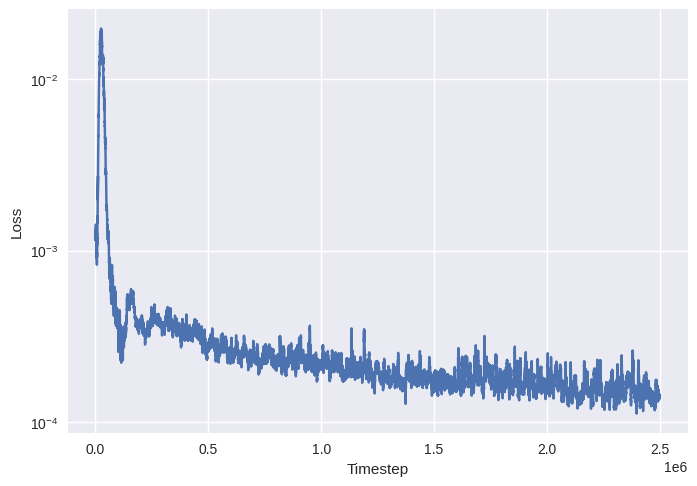
\includegraphics[scale=0.5]{../ER_20spin/eco/min_cover/network/loss.png}

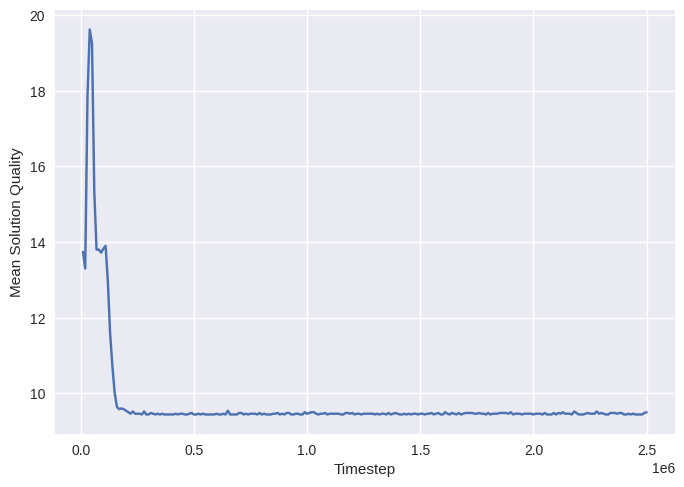
\includegraphics[scale=0.5]{../ER_20spin/eco/min_cover/network/training_curve.png}

\textbf{Still need to run actual tests, this is only training results, which are promising but not conclusive.}

\subsection{Generalization}

\textbf{Just some footnotes/brainstorming for now}

To generalize these ideas to any problem, some framework needs to be solidified for choosing observations and rewards. Something related to the constraints of the problem (if any) would need to be specified. For Minimum Vertex Cover there's a simple way of doing this as described in it's section, but extending this to other problems is more difficult. Further, there's no real way that I know of that could actually confirm whether other frameworks for learning would actually yield good results other than manually verifying it by creating the observations and reward mechanism then training a network (obviously bad and not very useful).

Definitely problems arise if the decision isn't binary, adding or removing a vertex from a single solution set, like with Minimum K-Cut. For a problem like the Traveling Salesman Problem, there's the issue that the solution isn't just splitting the graph into two sets, but is instead an ordered list. 

\bibliography{main}
\bibliographystyle{ieeetr}


\end{document}